\section{Evaluation}
\label{sec:evaluation}

\subsection{Experimental setup}
\paragraph{Dataset.}
We evaluate \critical on the public VE-Bench benchmark~\cite{vebench}, constructing 986 pairwise comparisons of candidate video edits across 128 source-video groups with human preference labels. Comparison features combine counterbalanced native-video judgments, contact-sheet frame judgments, and multi-agent debate factors, with binary missingness masks tracking unavailable modalities.

\paragraph{Validation protocol and baselines.}
All experiments use five-fold source-grouped cross-validation (repeated across five split seeds) so that edits sharing the same source video never appear in both training and test splits. Feature normalization, calibration weights $\beta$, and routing thresholds are fitted strictly on training folds and evaluated via pooled out-of-fold predictions. We report human-agreement accuracy (with 95\% grouped-bootstrap confidence intervals resampling source groups) and compare the unified \critical router against four baselines: (1)~the primary native-video judge, (2)~the stronger secondary native-video judge, (3)~a random-routing control, and (4)~a two-expert native-video router.

\begin{figure}[t]
\centering
% Full-coverage VE-Bench fusion accuracy (single-column TikZ figure).
\begingroup
\definecolor{evInk}{HTML}{202830}
\definecolor{evMuted}{HTML}{56616B}
\definecolor{evGrid}{HTML}{DCE3E8}
\definecolor{evAxis}{HTML}{77848C}
\definecolor{evBlue}{HTML}{246083}
\definecolor{evTeal}{HTML}{23675B}
\definecolor{evGrey}{HTML}{7C8993}
\resizebox{\columnwidth}{!}{%
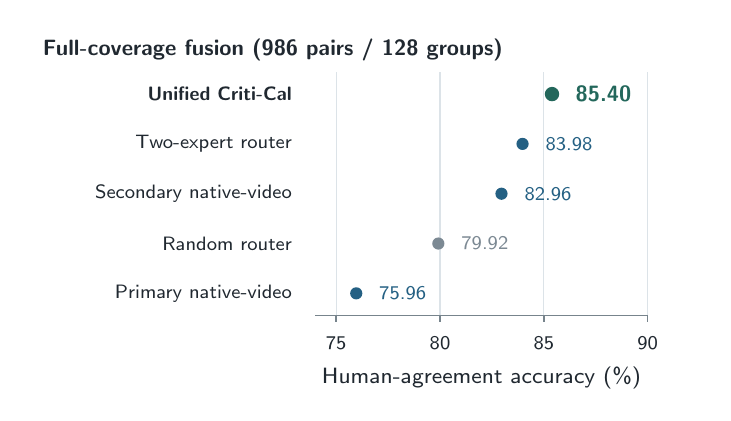
\begin{tikzpicture}[
  x=1pt,y=1pt,
  evlabel/.style={anchor=east,font=\sffamily\fontsize{7.5}{9}\selectfont,text=evInk},
  evtick/.style={anchor=north,font=\sffamily\fontsize{7.2}{8.6}\selectfont,text=evInk},
  evval/.style={anchor=west,font=\sffamily\fontsize{7.4}{8.8}\selectfont}
]
\path[use as bounding box] (0,-24) rectangle (244,108);

% Plot area: x in [104, 224] maps accuracy [74, 90] -> x = 104 + (acc - 74) * 7.5
% y rows: 0->12, 1->30, 2->48, 3->66, 4->84
\foreach \acc/\xpos in {75/111.5, 80/149.0, 85/186.5, 90/224.0} {
  \draw[evGrid,line width=0.5pt] (\xpos,4) -- (\xpos,92);
  \draw[evAxis,line width=0.6pt] (\xpos,4) -- (\xpos,1.5);
  \node[evtick] at (\xpos,0) {\acc};
}
\draw[evAxis,line width=0.6pt] (104,4) -- (224,4);
\node[anchor=north,font=\sffamily\fontsize{7.8}{9.2}\selectfont,text=evInk] at (164,-11)
  {Human-agreement accuracy (\%)};

% Row 0: Primary native-video (75.96%) -> x = 118.73
\node[evlabel] at (99,12) {Primary native-video};
\fill[evBlue] (118.73,12) circle (2.2pt);
\node[evval,text=evBlue] at (123.5,12) {75.96};

% Row 1: Random router (79.92%) -> x = 148.39
\node[evlabel] at (99,30) {Random router};
\fill[evGrey] (148.39,30) circle (2.2pt);
\node[evval,text=evGrey] at (153.2,30) {79.92};

% Row 2: Secondary native-video (82.96%) -> x = 171.21
\node[evlabel] at (99,48) {Secondary native-video};
\fill[evBlue] (171.21,48) circle (2.2pt);
\node[evval,text=evBlue] at (176.0,48) {82.96};

% Row 3: Two-expert router (83.98%) -> x = 178.82
\node[evlabel] at (99,66) {Two-expert router};
\fill[evBlue] (178.82,66) circle (2.2pt);
\node[evval,text=evBlue] at (183.6,66) {83.98};

% Row 4: Unified Criti-Cal (85.40%) -> x = 189.47
\node[evlabel,font=\sffamily\fontsize{7.5}{9}\selectfont\bfseries] at (99,84) {Unified \textsc{Criti-Cal}};
\fill[evTeal] (189.47,84) circle (2.6pt);
\node[evval,text=evTeal,font=\sffamily\fontsize{7.6}{9}\selectfont\bfseries] at (194.5,84) {85.40};

\node[anchor=west,font=\sffamily\fontsize{8.2}{9.6}\selectfont\bfseries,text=evInk] at (2,100)
  {Full-coverage fusion (986 pairs / 128 groups)};
\end{tikzpicture}%
}
\endgroup

\caption{Full-coverage pairwise human-agreement accuracy on VE-Bench across individual judges, routing controls, and the unified \critical router.}
\Description{Full-coverage accuracy is 75.96 percent for the primary native-video judge, 79.92 for a random router, 82.96 for the secondary native-video judge, 83.98 for a two-expert router, and 85.40 for the unified Criti-Cal router.}
\label{fig:fusion-accuracy}
\end{figure}

\subsection{Full-coverage fusion results}
Figure~\ref{fig:fusion-accuracy} compares full-coverage pairwise accuracy across all evaluated configurations on VE-Bench. A single primary native-video judge achieves 75.96\% human agreement, while the stronger secondary native-video judge reaches 82.96\% and a two-expert router over both video judges reaches 83.98\% (versus 79.92\% for random expert routing). Incorporating complementary contact-sheet frame judgments and grounded debate features in the unified \critical router raises full-coverage accuracy to \textbf{85.40\%}---gaining $+9.44$ percentage points over the primary video judge, $+2.43$ points over the strongest single video judge (95\% grouped-bootstrap CI $[0.95, 4.04]$), and $+1.42$ points over the two-expert video router (95\% CI $[0.21, 2.71]$). Comparing against the stronger video judge and two-expert router confirms that the gain comes from cross-modal perception and grounded features rather than simply replacing a weaker judge.

% Balance the final page from its first column.
\begin{figure}[t]
\centering
% Selective routing curve on VE-Bench (single-column TikZ figure).
\begingroup
\definecolor{evInk}{HTML}{202830}
\definecolor{evMuted}{HTML}{56616B}
\definecolor{evGrid}{HTML}{DCE3E8}
\definecolor{evAxis}{HTML}{77848C}
\definecolor{evBlue}{HTML}{246083}
\resizebox{\columnwidth}{!}{%
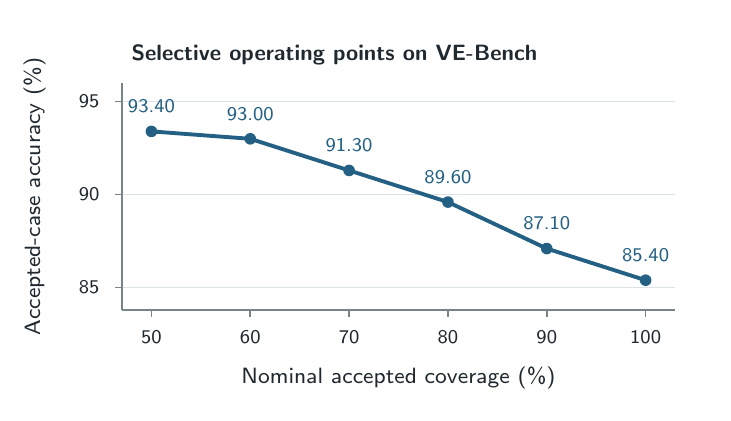
\begin{tikzpicture}[
  x=1pt,y=1pt,
  evtickx/.style={anchor=north,font=\sffamily\fontsize{7.2}{8.6}\selectfont,text=evInk},
  evticky/.style={anchor=east,font=\sffamily\fontsize{7.2}{8.6}\selectfont,text=evInk},
  evpt/.style={anchor=south,font=\sffamily\fontsize{7.1}{8.5}\selectfont,text=evBlue}
]
\path[use as bounding box] (0,-24) rectangle (244,108);

% Plot area:
% x: coverage in [47, 103] -> [34, 234] => x = 34 + (cov - 47) * (200 / 56)
% y: accuracy in [83.8, 96.0] -> [6, 88] => y = 6 + (acc - 83.8) * (82 / 12.2)
\foreach \acc/\ypos in {85/14.07, 90/47.67, 95/81.28} {
  \draw[evGrid,line width=0.5pt] (34,\ypos) -- (234,\ypos);
  \draw[evAxis,line width=0.6pt] (34,\ypos) -- (31.5,\ypos);
  \node[evticky] at (29.5,\ypos) {\acc};
}
\foreach \cov/\xpos in {50/44.71, 60/80.43, 70/116.14, 80/151.86, 90/187.57, 100/223.29} {
  \draw[evAxis,line width=0.6pt] (\xpos,6) -- (\xpos,3.5);
  \node[evtickx] at (\xpos,2) {\cov};
}
\draw[evAxis,line width=0.6pt] (34,6) -- (34,88);
\draw[evAxis,line width=0.6pt] (34,6) -- (234,6);

\node[anchor=north,font=\sffamily\fontsize{7.8}{9.2}\selectfont,text=evInk] at (134,-11)
  {Nominal accepted coverage (\%)};
\node[rotate=90,anchor=south,font=\sffamily\fontsize{7.8}{9.2}\selectfont,text=evInk] at (10,47)
  {Accepted-case accuracy (\%)};

% Points:
% (50, 93.4)  -> (44.71, 70.52)
% (60, 93.0)  -> (80.43, 67.84)
% (70, 91.3)  -> (116.14, 56.41)
% (80, 89.6)  -> (151.86, 44.98)
% (90, 87.1)  -> (187.57, 28.18)
% (100, 85.4) -> (223.29, 16.75)
\draw[evBlue,line width=1.4pt]
  (44.71,70.52) -- (80.43,67.84) -- (116.14,56.41) --
  (151.86,44.98) -- (187.57,28.18) -- (223.29,16.75);

\foreach \xp/\yp/\lbl in {
  44.71/70.52/93.40,
  80.43/67.84/93.00,
  116.14/56.41/91.30,
  151.86/44.98/89.60,
  187.57/28.18/87.10,
  223.29/16.75/85.40
} {
  \fill[evBlue] (\xp,\yp) circle (2.1pt);
  \node[evpt] at (\xp,\yp+3.2) {\lbl};
}

\node[anchor=west,font=\sffamily\fontsize{8.2}{9.6}\selectfont\bfseries,text=evInk] at (34,98)
  {Selective operating points on VE-Bench};
\end{tikzpicture}%
}
\endgroup

\caption{Selective accuracy on VE-Bench across accepted coverage levels when deferring high-risk comparisons via the reliability gate.}
\Description{Accepted-case accuracy is 93.40, 93.00, 91.30, 89.60, 87.10, and 85.40 percent at nominal coverage 50, 60, 70, 80, 90, and 100 percent.}
\label{fig:selective-routing}
\end{figure}

\subsection{Selective prediction}
When the reliability gate (Section~\ref{sec:gate}) is enabled, comparisons are ranked by risk score $r_i$ and pairs exceeding the acceptance threshold are deferred~\cite{geifman2017selective,madras2018predict}, trading \emph{accepted coverage} (the fraction of pairs decided automatically) for higher \emph{selective accuracy} (human agreement on the accepted subset). As shown in Figure~\ref{fig:selective-routing}, deferring the highest-risk comparisons steadily increases human agreement on the accepted subset: accuracy rises from 85.40\% at 100\% coverage to 87.10\% (90\% coverage), 89.60\% (80\%), 91.30\% (70\%), 93.00\% (60\%), and \textbf{93.40\%} when retaining the most reliable 50\% of comparisons. In practice, ($t_{\mathrm{accept}}$, $t_{\mathrm{investigate}}$) can be tuned on training groups to match review capacity, resolving low-risk pairs in one pass while reserving deliberation and human review for high-risk cases.
